\section{Complexity}

In this section, we come up with a rough estimate of the cost of the
MLFMM and an asymptotic estimate of its cost. The FMM used in our
implementation consists of several different parts, which can be
considered independently:
\begin{itemize}
\item The $\SSmat$, $\SRmat$, and $\RRmat$ translations.
\item The construction of $S$ factorizations for the finest boxes.
\item Direct evaluation.
\item Indirect evaluation.
\end{itemize}
We will consider each of these items in turn. Important quantities
related to the algorithm are as follows:
\begin{center}
  \begin{tabular}{cl}
    $\fmmdepth$ & The maximum FMM depth. \\
    $\bandlimit$ & The bandlimit of the function $\bandfunc$. \\
    $\neighborhoodradius$ & The integer neighborhood radius. \\
    $\bandlimit\neighborhoodradius$ & The number of source points for the FMM (due to periodic tiling).\@ \\
    $\numarbpts$ & The number of evaluation points (interpolation nodes $\arbpt{\arbptindex}$). \\
    $\truncnum$ & The truncation number of the kernel approximation.
  \end{tabular}
\end{center}
We also note that in our estimate of the complexity, we assume that
the source and evaluation points are distributed uniformly. We note
that assumption of uniformity, while generally useful, can be improved
upon for the interpolation nodes. In particular, the integer
neighborhood radius $\neighborhoodradius$ plays a larger role: if we
ignore the checkpoints, the evaluation points only occur in the range
$[\tfrac{n}{2n+1}, \tfrac{n+1}{2n+1})$.  If the FMM is implemented to
take advantage of this, the number of translation operators that must
be applied can be significantly reduced. The implementation used in
the current work does not take advantage of this optimization.

Applying the $\SSmat, \SRmat$, and $\RRmat$ translation operators
takes approximately $O(\truncnum^2)$ operations, as applying these
operators corresponds to multiplication of a vector in $\C^\truncnum$
by a matrix in $\C^{\truncnum\times\truncnum}$. With the parameter
$\fmmdepth$ chosen, a union of four perfect binary trees of height
$\fmmdepth - 1$ is constructed---this data structure will be referred
to as a translation hierarchy (see Figure~\ref{fig:fmm} for a
graphical depiction of the case of $\fmmdepth = 4$). For each
subinterval at the finest level of subdivision, the FMM involves a
hierarchical sequence of translations such that the function can be
efficiently evaluated in this subinterval using an $R$ expansion. We
will not dwell on the details of this, as they can readily be found
elsewhere~\cite{fmm-helmholtz, fmm-orig}.

To estimate the cost of the one-dimensional FMM, we start by
determining the cost of the translation operators. As the translation
hierarchy consists of four perfect binary trees of height
$\fmmdepth - 1$, since one $\SSmat$ and one $\RRmat$ translation operator is
computed for each edge in this tree, and since there are
$2^{\fmmdepth-1} - 2$ edges in a perfect binary tree of the given
height, the combined cost of the $\SSmat$ and $\RRmat$ translation operators
is $8(2^{\fmmdepth-1} - 2)O(\truncnum^2) =
O(2^\fmmdepth\truncnum^2)$. As for the $\SRmat$ translation operators,
we note for each node in the translation hierarchy, at most (and in
most cases) three $\SRmat$ operators are computed (cf.\
Figure~\ref{fig:fmm}). Since there are $4(2^{\fmmdepth-1}-1)$ nodes in
the translation hierarchy, the cost of applying the $\SRmat$ operators is
$12(2^{\fmmdepth-1}-1)O(\truncnum^2) =
O(2^\fmmdepth\truncnum^2)$. Then, the overall cost of applying the
translation operators is $O(2^\fmmdepth\truncnum^2)$.

The cost of the rest of the phases of the algorithm is straightforward
to estimate. The construction of the $S$-factorizations is asymptotic
in the number of source points and the truncation number, so the
corresponding cost is
$O(\bandlimit\truncnum\neighborhoodradius)$. Indirect evaluation at a
single point is $O(\truncnum)$ (evaluating a polynomial of degree
$\truncnum$), and the entire indirect evaluation phase takes place at
$\numarbpts$ points, so the overall cost is
$O(\numarbpts\truncnum)$. Finally, the direct evaluation cost is
proportional to the number of points in the 1-cell neighborhood of
each cell containing a target point times the number of target
points---since the number of source points that align with target
points is $\bandlimit$, the overall cost is proportional to
$2^{-L} \bandlimit \numarbpts$.

\begin{figure}[h]
  \centering
  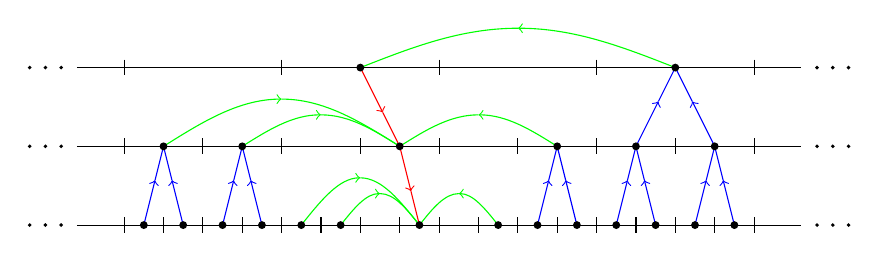
\begin{tikzpicture}[scale = 2.0]
  \def \cdotssizes{0.0125};
  \def \cdotspacing{0.1};
  \def \nodesize{0.025};
  \def \leftextent{0};
  \def \rightextent{4};
  \def \hmargin{0.3};
  \def \hrulertickheight{0.1};
  \def \yone {0.0};
  \def \ytwo {0.5};
  \def \ythree {1.0};
  \def \yfour {1.5};

  % Draw horizontal rulers and cdots on the sides.
  \foreach \y in {\yone, \ytwo, \ythree} {
    \draw [-] ({\leftextent - \hmargin}, \y) -- ({\rightextent + \hmargin}, \y);
    \foreach \i in {1, 2, 3} {
      \fill[black] ({\leftextent - \hmargin - (\i * \cdotspacing)}, \y) circle (\cdotssizes);
      \fill[black] ({\rightextent + \hmargin + (\i * \cdotspacing)}, \y) circle (\cdotssizes);
    }
  };
  
  % Draw ticks on each horizontal ruler.
  \foreach \x in {\leftextent, 1.0, ..., \rightextent} {
    \draw [-] (\x, {\ythree + (\hrulertickheight / 2)}) -- (\x, {\ythree - (\hrulertickheight / 2)});
  };
  \foreach \x in {\leftextent, 0.5, ..., \rightextent} {
    \draw [-] (\x, {\ytwo + (\hrulertickheight / 2)}) -- (\x, {\ytwo - (\hrulertickheight / 2)});
  };
  \foreach \x in {\leftextent, 0.25, ..., \rightextent} {
    \draw [-] (\x, {\yone + (\hrulertickheight / 2)}) -- (\x, {\yone - (\hrulertickheight / 2)});
  };
  
  % Draw SS translation arrows.
  \def \theta {4/7}
  \foreach \x in {0.25, 0.75, 2.75, 3.25, 3.75} {
    \def \midpt {(1 - \theta) * \yone + \theta * \ytwo};
    \draw [-, blue] (\x, \ytwo) -- ({\x - 0.125*(1 - \theta)}, {\midpt});
    \draw [<-, blue] ({\x - 0.125*(1 - \theta)}, {\midpt}) -- ({\x - 0.125}, \yone);
    \draw [-, blue] (\x, \ytwo) -- ({\x + 0.125*(1 - \theta)}, {\midpt});
    \draw [<-, blue] ({\x + 0.125*(1 - \theta)}, {\midpt}) -- ({\x + 0.125}, \yone);
  };
  \foreach \x in {3.5} {
    \def \midpt {(1 - \theta) * \ytwo + \theta * \ythree};
    \draw [-, blue] (\x, \ythree) -- ({\x - 0.25*(1 - \theta)}, {\midpt});
    \draw [<-, blue] ({\x - 0.25*(1 - \theta)}, {\midpt}) -- ({\x - 0.25}, \ytwo);
    \draw [-, blue] (\x, \ythree) -- ({\x + 0.25*(1 - \theta)}, {\midpt});
    \draw [<-, blue] ({\x + 0.25*(1 - \theta)}, {\midpt}) -- ({\x + 0.25}, \ytwo);
  };
  
  % Draw RR translation arrows.
  \def \theta {3/7}
  \foreach \x in {1.75} {
    \def \midpt {(1 - \theta) * \yone + \theta * \ytwo};
    \draw [->, red] (\x, \ytwo) -- ({\x + 0.125*(1 - \theta)}, {\midpt});
    \draw [-, red] ({\x + 0.125*(1 - \theta)}, {\midpt}) -- ({\x + 0.125}, \yone);
  };
  \foreach \x in {1.5} {
    \def \midpt {(1 - \theta) * \ytwo + \theta * \ythree};
    \draw [->, red] (\x, \ythree) -- ({\x + 0.25*(1 - \theta)}, {\midpt});
    \draw [-, red] ({\x + 0.25*(1 - \theta)}, {\midpt}) -- ({\x + 0.25}, \ytwo);
  };

  % Draw SR translation arrows.
  \def \center {1.5}
  \foreach \x in {3.5} {
    \pgfmathsetmacro{\xmid}{(\center + \x)/2};
    \pgfmathsetmacro{\ymid}{(\ythree + \yfour)/2};
    \draw[->, green] (\x, \ythree) sin (\xmid, \ymid);
    \draw[-, green] (\xmid, \ymid) cos (\center, \ythree);
  };
  \def \center {1.75}
  \pgfmathsetmacro{\maxdist}{abs(\center - 0.25)};
  \foreach \x in {0.25, 0.75, 2.75} {
    \pgfmathsetmacro{\dist}{abs(\center - \x)};
    \pgfmathsetmacro{\theta}{0.6 * \dist / abs(\maxdist)};
    \pgfmathsetmacro{\xmid}{(\center + \x)/2};
    \pgfmathsetmacro{\ymid}{(1 - \theta) * \ytwo + \theta * \ythree};
    \draw[->, green] (\x, \ytwo) sin (\xmid, \ymid);
    \draw[-, green] (\xmid, \ymid) cos (\center, \ytwo);
  };
  \def \center {1.875}
  \pgfmathsetmacro{\maxdist}{abs(\center - 1.125)};
  \foreach \x in {1.125, 1.375, 2.375} {
    \pgfmathsetmacro{\dist}{abs(\center - \x)};
    \pgfmathsetmacro{\theta}{0.6 * \dist / abs(\maxdist)};
    \pgfmathsetmacro{\xmid}{(\center + \x)/2};
    \pgfmathsetmacro{\ymid}{(1 - \theta) * \yone + \theta * \ytwo};
    \draw[->, green] (\x, \yone) sin (\xmid, \ymid);
    \draw[-, green] (\xmid, \ymid) cos (\center, \yone);
  };
  
  % Draw node circles.
  \foreach \x in {1.5, 3.5} {
    \fill[black] (\x, \ythree) circle (\nodesize);
  };
  \foreach \x in {0.25, 0.75, 1.75, 2.75, 3.25, 3.75} {
    \fill[black] (\x, \ytwo) circle (\nodesize);
  };
  \foreach \x in {0.125, 0.375, 0.625, 0.875, 1.125, 1.375, 1.875, 2.375, 2.625, 2.875, 3.125, 3.375, 3.625, 3.875} {
    \fill [black] (\x, \yone) circle (\nodesize);
  };
\end{tikzpicture} \\

%%% Local Variables:
%%% mode: latex
%%% TeX-master: "../paper/paper"
%%% End:

  \caption{an illustration of the translation phases of the
    one-dimensional FMM.}\label{fig:fmm}
\end{figure}

\begin{figure}[h]
  \centering
  \begin{tikzpicture}
  \begin{axis}[
    xmode=log,
    zmode=log,
    view/az=-30,
    xlabel={$K$},
    ylabel={$L$},
    zlabel={Time (s)},
    legend entries={NUFFT Runtime, Optimum},
    legend style={
      at={(1.03, 0.5)},
      anchor=west
    }]
    \addplot3[surf] file {../../py/new/data_optL.dat};
    \addplot3+[only marks] file {../../py/new/data_optL_argmins.dat};
  \end{axis}
\end{tikzpicture}

  \caption{test}\label{fig:optL}
\end{figure}

% Local Variables:
% TeX-master: "../paper.tex"
% indent-tabs-mode: nil
% End:
